\section{Presentación de los Resultados}

\subsection{Distribución de los antipatrones detectados}

Los 445 hallazgos se distribuyen de forma marcadamente desigual entre los cuatro antipatrones implementados. La Tabla~\ref{tab:distribucion} muestra que AP1, \emph{Hardcoded Prompt Infiltration}, concentra 273 hallazgos (61,35\,\%) en 20 repositorios; AP5, \emph{Non-Deterministic Exception Suppression}, concentra 152 (34,16\,\%) en 14 repositorios; AP3, \emph{Hardcoded Provider Lock-in}, registra 17 (3,82\,\%) en 6 repositorios; y AP4, \emph{Monolithic RAG Function}, registra 3 (0,67\,\%) en 3 repositorios. AP2 y AP6 no aparecen en la tabla porque no fueron implementados: no se evaluaron y no debe interpretarse su ausencia como prevalencia cero.

\begin{table}[t]
\centering
\scriptsize
\setlength{\tabcolsep}{3pt}
\caption{Distribución de los hallazgos detectados por antipatrón}
\label{tab:distribucion}
\begin{tabularx}{\columnwidth}{@{}l >{\raggedright\arraybackslash}X r r r l@{}}
\toprule
\textbf{ID} & \textbf{Antipatrón} & \textbf{Hall.} & \textbf{\%} & \textbf{Rep.} & \textbf{Estado} \\
\midrule
\textbf{AP1} & Hardcoded Prompt Infiltration & 273 & 61,35 & 20 & Impl. \\
\textbf{AP2} & Vector Store Leakage & --- & --- & --- & No eval. \\
\textbf{AP3} & Hardcoded Provider Lock-in & 17 & 3,82 & 6 & Impl. \\
\textbf{AP4} & Monolithic RAG Function & 3 & 0,67 & 3 & Impl. \\
\textbf{AP5} & Non-Deterministic Exception Suppression & 152 & 34,16 & 14 & Impl. \\
\textbf{AP6} & Unvalidated Generation Output & --- & --- & --- & No eval. \\
\midrule
\textbf{Total} & & 445 & 100,00 & 21 & 4 de 6 \\
\bottomrule
\end{tabularx}
\end{table}

La diferencia entre AP1 y AP4 es de dos órdenes de magnitud. Esta diferencia puede reflejar tanto una presencia real desigual de los fenómenos como una sensibilidad distinta de las reglas. AP1 se activa con una condición relativamente común en aplicaciones que incorporan prompts en el código; AP4 exige una función de más de sesenta líneas que combine recuperación y generación, una construcción menos frecuente y más fácil de fragmentar en funciones auxiliares. La distribución observada no permite separar ambos factores, y por ello el informe no compara la prevalencia relativa de los antipatrones como si midiera una única propiedad del dominio.

\subsection{Hallazgos por repositorio y concentración}

La Figura~\ref{fig:repositorios} ordena los 23 repositorios por número total de hallazgos y descompone cada barra por antipatrón. Dos repositorios dominan la distribución: \texttt{multimindlab/multimind-sdk} con 194 hallazgos y \texttt{bojieli/ai-agent-book} con 86. Juntos representan 280 de 445 hallazgos (62,9\,\%). Les siguen \texttt{ai-bot-pro/achatbot} con 27, \texttt{headroomlabs-ai/headroom} y \texttt{run-llama/llama\_index} con 21 cada uno, y \texttt{hoangsonww/Agentic-AI-Pipeline} con 15. En el extremo opuesto, 21 repositorios tienen al menos un hallazgo, mientras que \texttt{ZhishaBai-web/help-you-find-job} (8 módulos) y \texttt{LibreChat-AI/rag-api} (22 módulos) no registran ninguno.

\begin{figure*}[t]
\centering
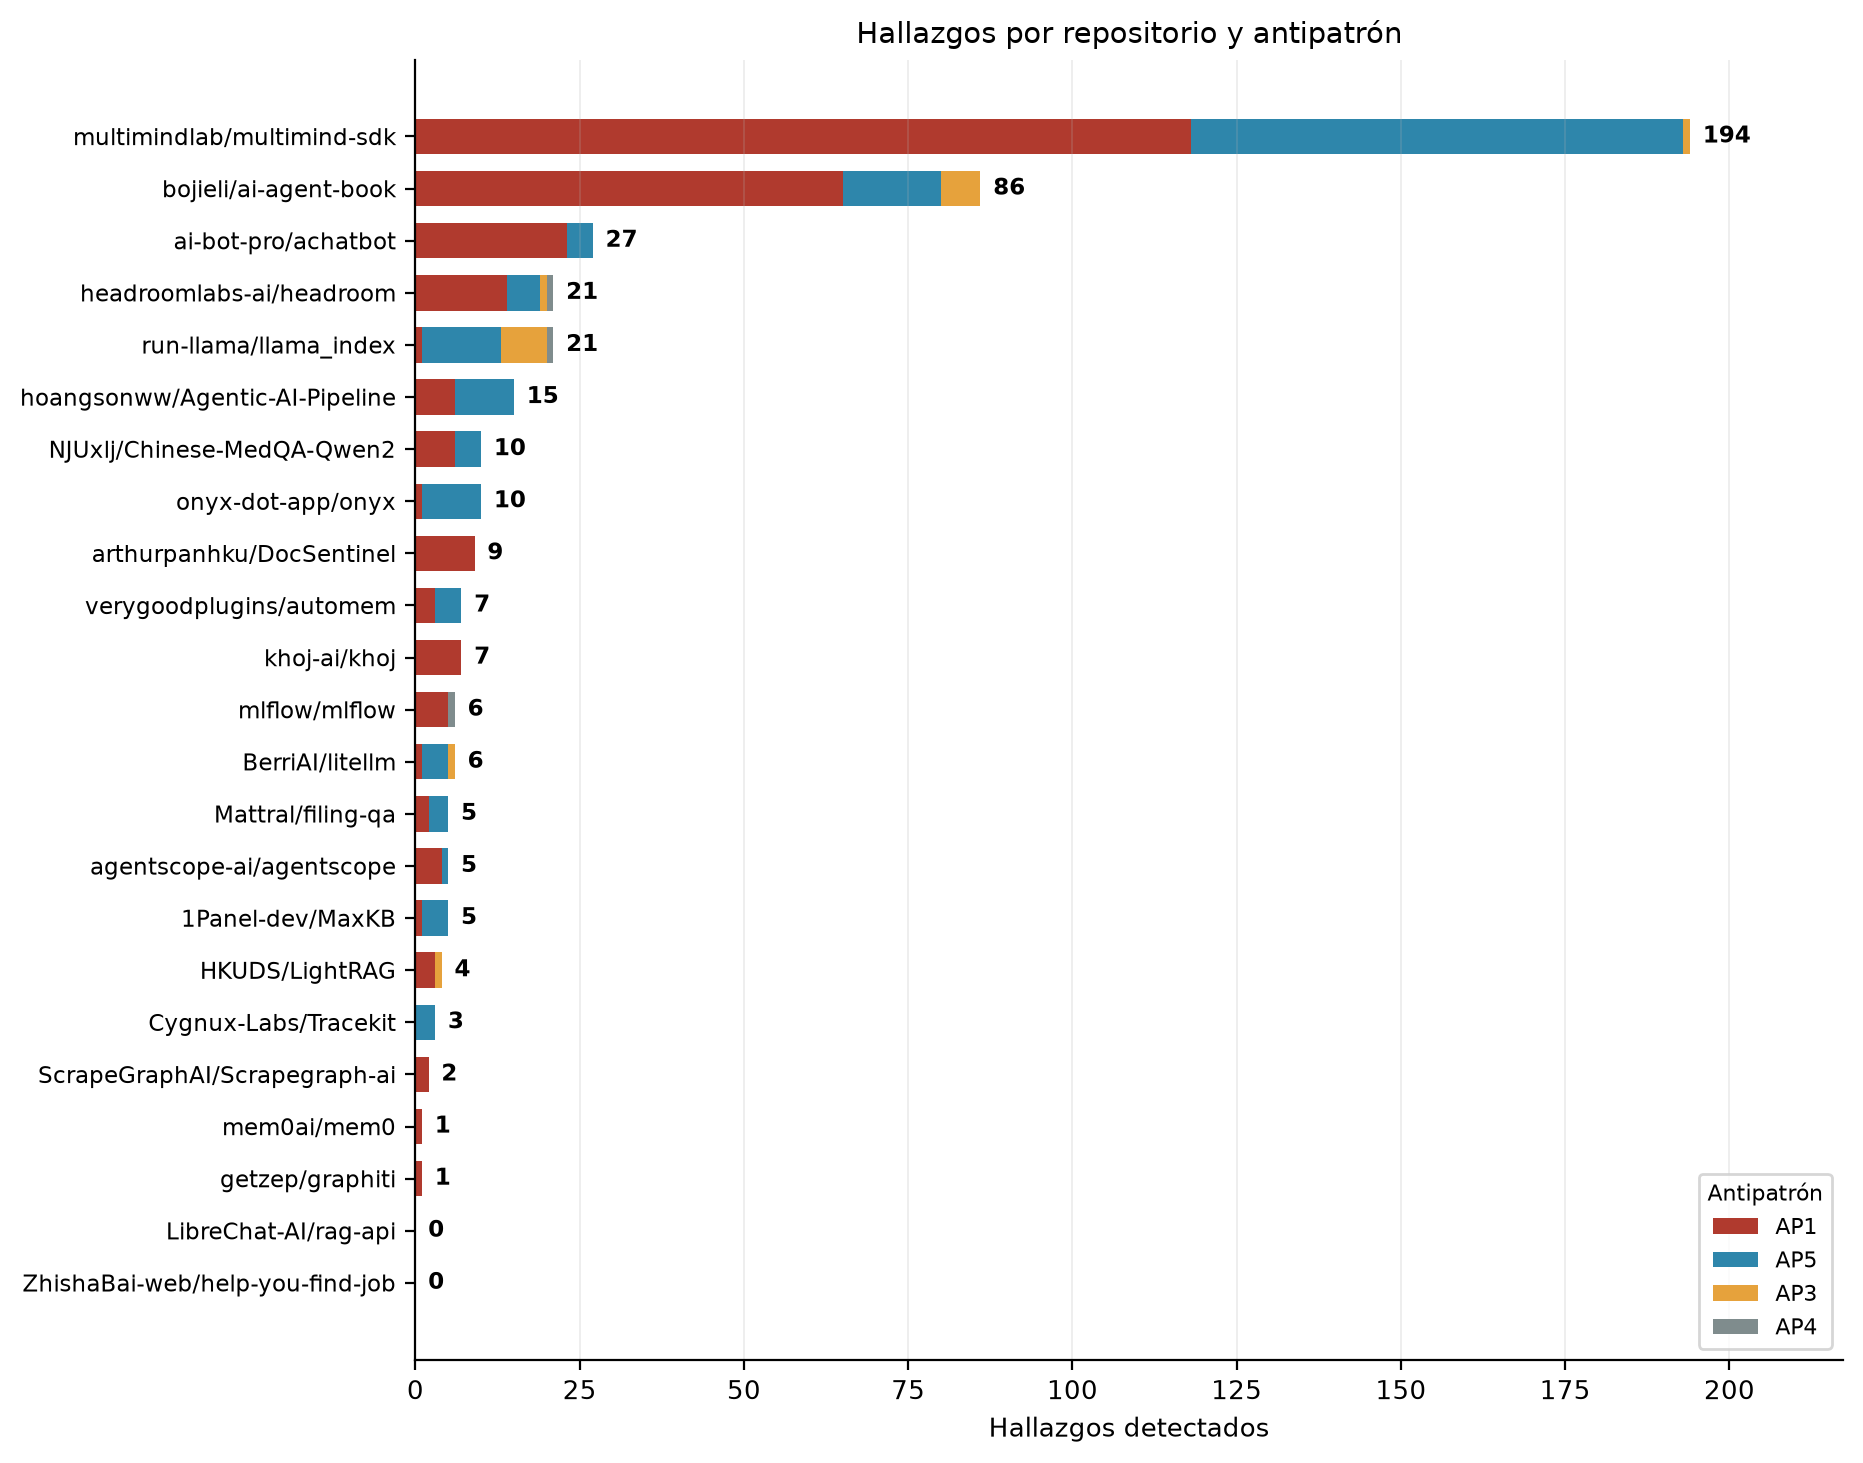
\includegraphics[width=0.90\textwidth]{figuras/fig04_hallazgos_por_repositorio.png}
\caption{Hallazgos por repositorio y antipatrón. Los repositorios se ordenan por número total de hallazgos. Los dos repositorios sin hallazgos aparecen al final con valor cero.}
\label{fig:repositorios}
\end{figure*}

La concentración tiene dos consecuencias. Primero, los contrastes globales están influidos por unos pocos repositorios: si \texttt{multimindlab/multimind-sdk} se comporta de forma atípica, su peso en el total puede arrastrar las comparaciones. Segundo, la unidad de observación independiente no es el módulo sino, en el mejor de los casos, el repositorio, y con solo dos repositorios sin hallazgos no es posible una comparación agregada estable. El análisis de sensibilidad por repositorio, presentado más adelante, confirma esta dificultad.

También es relevante que el repositorio con más hallazgos no sea el más grande. \texttt{multimindlab/multimind-sdk} tiene 392 módulos, frente a 3601 de \texttt{BerriAI/litellm} o 2440 de \texttt{onyx-dot-app/onyx}. Su tasa de módulos con antipatrón es 10,71\,\%, la más alta de la muestra, mientras que la de \texttt{BerriAI/litellm} es 0,14\,\%. Esta diferencia sugiere que la densidad de antipatrones depende de prácticas de diseño y no solo del tamaño del repositorio, aunque el diseño transversal no permite atribuir la diferencia a una causa específica.

\subsection{Estadística descriptiva}

La Tabla~\ref{tab:descriptivos} reporta media, desviación estándar, mediana, cuartiles y extremos para las cinco métricas en los grupos \emph{todos}, \emph{con AP} y \emph{sin AP}. Las distribuciones son asimétricas y presentan valores extremos, de modo que la mediana es un resumen más informativo que la media. En \texttt{cc\_max}, la mediana pasa de 5 en el grupo sin antipatrones a 14 en el grupo con antipatrones; en \texttt{mi}, de 68,04 a 39,74; en \texttt{cbo\_mod}, de 2 a 3; y en \texttt{sloc}, de 87 a 399. Las medias siguen la misma dirección, pero son considerablemente mayores en el grupo con antipatrones, especialmente en \texttt{sloc} (614,05 frente a 204,04), lo que evidencia la cola de módulos grandes.

\begin{table*}[t]
\centering
\footnotesize
\setlength{\tabcolsep}{5pt}
\caption{Estadística descriptiva de las métricas por grupo}
\label{tab:descriptivos}
\begin{tabularx}{\textwidth}{@{}X l r r r r r r r r@{}}
\toprule
\textbf{Métrica} & \textbf{Grupo} & \textbf{n} & \textbf{Media} & \textbf{DE} & \textbf{Mediana} & \textbf{Q1} & \textbf{Q3} & \textbf{Mín.} & \textbf{Máx.} \\
\midrule
\texttt{cc\_max} & Todos & 15\,768 & 8,28 & 14,26 & 5,00 & 1,00 & 11,00 & 0,00 & 533,00 \\
\texttt{cc\_max} & Con AP & 201 & 22,35 & 28,48 & 14,00 & 9,00 & 24,00 & 1,00 & 227,00 \\
\texttt{cc\_max} & Sin AP & 15\,567 & 8,10 & 13,89 & 5,00 & 1,00 & 10,00 & 0,00 & 533,00 \\
\midrule
\texttt{mi} & Todos & 15\,768 & 68,47 & 27,20 & 67,57 & 49,09 & 100,00 & 0,00 & 100,00 \\
\texttt{mi} & Con AP & 201 & 38,09 & 20,32 & 39,74 & 25,71 & 51,79 & 0,00 & 100,00 \\
\texttt{mi} & Sin AP & 15\,567 & 68,87 & 27,06 & 68,04 & 49,46 & 100,00 & 0,00 & 100,00 \\
\midrule
\texttt{cbo\_mod} & Todos & 15\,768 & 2,20 & 2,06 & 2,00 & 1,00 & 3,00 & 0,00 & 43,00 \\
\texttt{cbo\_mod} & Con AP & 201 & 3,76 & 2,73 & 3,00 & 2,00 & 5,00 & 0,00 & 15,00 \\
\texttt{cbo\_mod} & Sin AP & 15\,567 & 2,18 & 2,04 & 2,00 & 1,00 & 3,00 & 0,00 & 43,00 \\
\midrule
\texttt{cc\_media} & Todos & 15\,768 & 2,95 & 3,06 & 2,43 & 1,00 & 4,01 & 0,00 & 120,00 \\
\texttt{cc\_media} & Con AP & 201 & 5,60 & 3,05 & 5,00 & 3,74 & 6,95 & 1,00 & 22,03 \\
\texttt{cc\_media} & Sin AP & 15\,567 & 2,92 & 3,04 & 2,38 & 1,00 & 4,00 & 0,00 & 120,00 \\
\midrule
\texttt{sloc} & Todos & 15\,768 & 209,27 & 478,66 & 89,00 & 26,00 & 224,00 & 0,00 & 13\,018,00 \\
\texttt{sloc} & Con AP & 201 & 614,05 & 983,40 & 399,00 & 209,00 & 660,00 & 21,00 & 10\,241,00 \\
\texttt{sloc} & Sin AP & 15\,567 & 204,04 & 466,38 & 87,00 & 25,00 & 219,00 & 0,00 & 13\,018,00 \\
\bottomrule
\end{tabularx}
\end{table*}

La comparación de medianas y medias revela el efecto de la asimetría. En \texttt{cc\_max}, la media del grupo con antipatrones (22,35) supera ampliamente su mediana (14), y su máximo alcanza 227; en \texttt{sloc}, la media (614,05) casi duplica la mediana (399) y el máximo llega a 10\,241. Estas diferencias justifican el uso de pruebas no paramétricas y de medidas de efecto basadas en rangos, y también advierten que una comparación de medias habría sobreestimado la separación entre grupos.

\subsection{Contraste primario}

La Tabla~\ref{tab:mann-whitney} presenta los tres contrastes primarios. Las tres métricas muestran diferencias estadísticamente significativas después de la corrección de Holm, con valores $p$ extremadamente pequeños y tamaños de efecto en la dirección esperada. En \texttt{cc\_max}, la mediana es 14 frente a 5, con $U=2\,517\,200{,}5$, $p_{Holm}=4{,}85\times10^{-50}$ y $\delta=+0{,}609$, un efecto grande. En \texttt{mi}, la mediana es 39,74 frente a 68,04, con $U=586\,956{,}5$, $p_{Holm}=2{,}00\times10^{-53}$ y $\delta=-0{,}625$, también un efecto grande. En \texttt{cbo\_mod}, la mediana es 3 frente a 2, con $U=2\,194\,635$, $p_{Holm}=7{,}41\times10^{-24}$ y $\delta=+0{,}403$, un efecto mediano.

\begin{table*}[t]
\centering
\footnotesize
\setlength{\tabcolsep}{4pt}
\caption{Contraste primario de Mann--Whitney U entre módulos con y sin antipatrones detectados}
\label{tab:mann-whitney}
\begin{tabularx}{\textwidth}{@{}X r r r r r l l r l@{}}
\toprule
\textbf{Métrica} & \textbf{n con} & \textbf{n sin} & \textbf{Med.\ con} & \textbf{Med.\ sin} & \textbf{U} & \textbf{p} & \textbf{p Holm} & \textbf{$\delta$} & \textbf{Magnitud} \\
\midrule
\texttt{cc\_max} & 201 & 15\,567 & 14,00 & 5,00 & 2\,517\,200,5 & $2{,}42 \times 10^{-50}$ & $4{,}85 \times 10^{-50}$ & $+0{,}609$ & Grande \\
\texttt{mi} & 201 & 15\,567 & 39,74 & 68,04 & 586\,956,5 & $6{,}68 \times 10^{-54}$ & $2{,}00 \times 10^{-53}$ & $-0{,}625$ & Grande \\
\texttt{cbo\_mod} & 201 & 15\,567 & 3,00 & 2,00 & 2\,194\,635,0 & $7{,}41 \times 10^{-24}$ & $7{,}41 \times 10^{-24}$ & $+0{,}403$ & Mediano \\
\bottomrule
\end{tabularx}
\end{table*}

La Figura~\ref{fig:metricas} ilustra las distribuciones mediante diagramas de caja. Los valores atípicos se omiten para facilitar la lectura, pero las medianas y los tamaños de efecto se conservan en la tabla. La separación visual es clara en las tres métricas: el grupo con antipatrones tiene cajas desplazadas hacia mayor complejidad, menor mantenibilidad y mayor acoplamiento. Sin embargo, la superposición entre grupos es considerable, especialmente en \texttt{cbo\_mod}, donde las cajas comparten buena parte de su rango. La existencia de una diferencia de grupo no implica que todos los módulos con antipatrón sean problemáticos ni que todos los módulos sin antipatrón estén sanos.

\begin{figure*}[t]
\centering
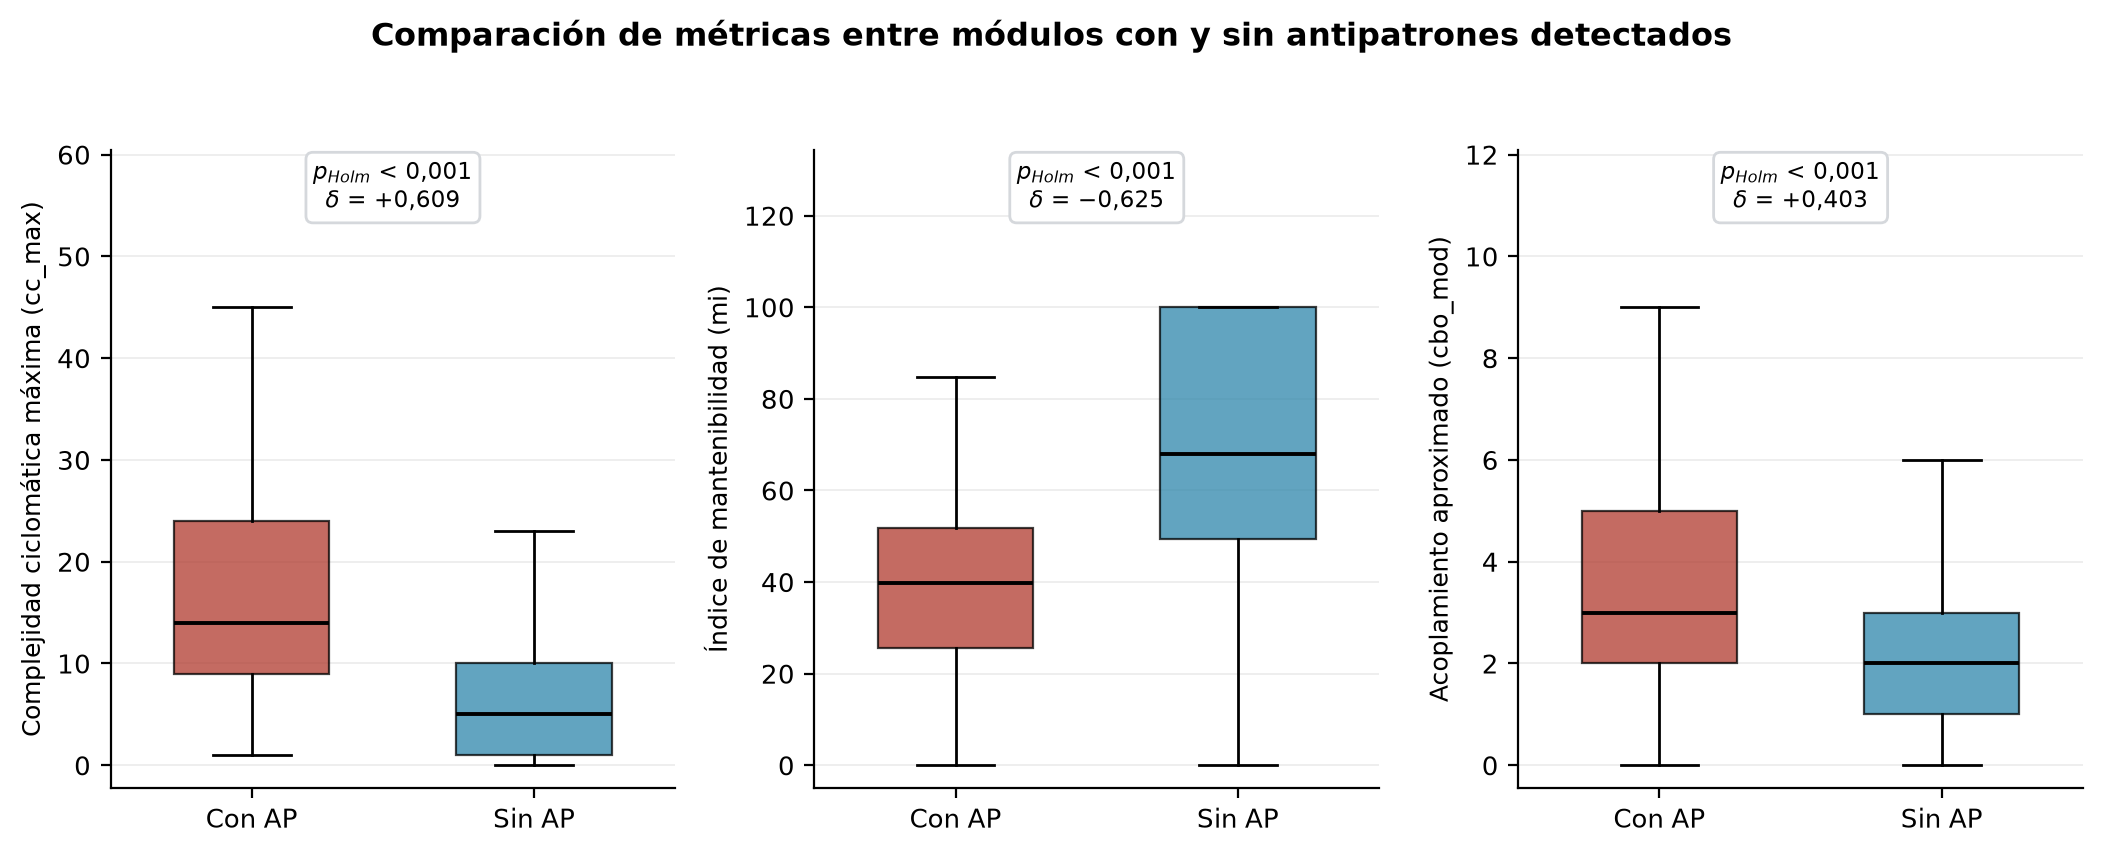
\includegraphics[width=0.95\textwidth]{figuras/fig05_comparacion_metricas.png}
\caption{Comparación de las tres métricas primarias entre módulos con y sin antipatrones detectados. Se omiten los valores atípicos para facilitar la lectura; las medianas y los tamaños de efecto se reportan en la Tabla~\ref{tab:mann-whitney}.}
\label{fig:metricas}
\end{figure*}

\subsection{Correlaciones de Spearman}

La Tabla~\ref{tab:spearman} presenta la asociación entre el número de hallazgos por módulo y las tres métricas primarias. Las tres correlaciones son estadísticamente significativas después de la corrección de Holm, pero de magnitud débil. \texttt{cc\_max} presenta $\rho=+0{,}119$ ($p_{Holm}=2{,}03\times10^{-50}$), \texttt{mi} presenta $\rho=-0{,}123$ ($p_{Holm}=6{,}78\times10^{-54}$) y \texttt{cbo\_mod} presenta $\rho=+0{,}080$ ($p_{Holm}=6{,}06\times10^{-24}$). Las direcciones coinciden con lo esperado: más hallazgos se asocian con mayor complejidad, menor mantenibilidad y mayor acoplamiento, pero la proporción de variación explicada es muy baja.

\begin{table*}[t]
\centering
\footnotesize
\setlength{\tabcolsep}{5pt}
\caption{Correlaciones de Spearman entre el número de hallazgos por módulo y las métricas}
\label{tab:spearman}
\begin{tabularx}{\textwidth}{@{}l r l l r >{\raggedright\arraybackslash}X@{}}
\toprule
\textbf{Métrica} & \textbf{$\rho$} & \textbf{p} & \textbf{p Holm} & \textbf{n} & \textbf{Lectura} \\
\midrule
\texttt{cc\_max} & $+0{,}119$ & $1{,}01 \times 10^{-50}$ & $2{,}03 \times 10^{-50}$ & 15\,768 & Asociación positiva débil \\
\texttt{mi} & $-0{,}123$ & $2{,}26 \times 10^{-54}$ & $6{,}78 \times 10^{-54}$ & 15\,768 & Asociación negativa débil \\
\texttt{cbo\_mod} & $+0{,}080$ & $6{,}06 \times 10^{-24}$ & $6{,}06 \times 10^{-24}$ & 15\,768 & Asociación positiva muy débil \\
\bottomrule
\end{tabularx}
\end{table*}

La Figura~\ref{fig:correlacion} muestra las distribuciones de cada métrica según el número de hallazgos por módulo, agrupado en cero, uno, dos, tres a cinco y seis o más. El grupo con cero hallazgos contiene 15\,567 módulos y domina la escala; los grupos con hallazgos son pequeños (129, 31, 23 y 18 módulos, respectivamente). Las medianas se desplazan en la dirección esperada, pero las cajas se superponen ampliamente y los grupos con más hallazgos no muestran una progresión monotónica perfecta. La correlación débil es consistente con esta imagen: hay una tendencia, no una relación estrecha.

\begin{figure*}[t]
\centering
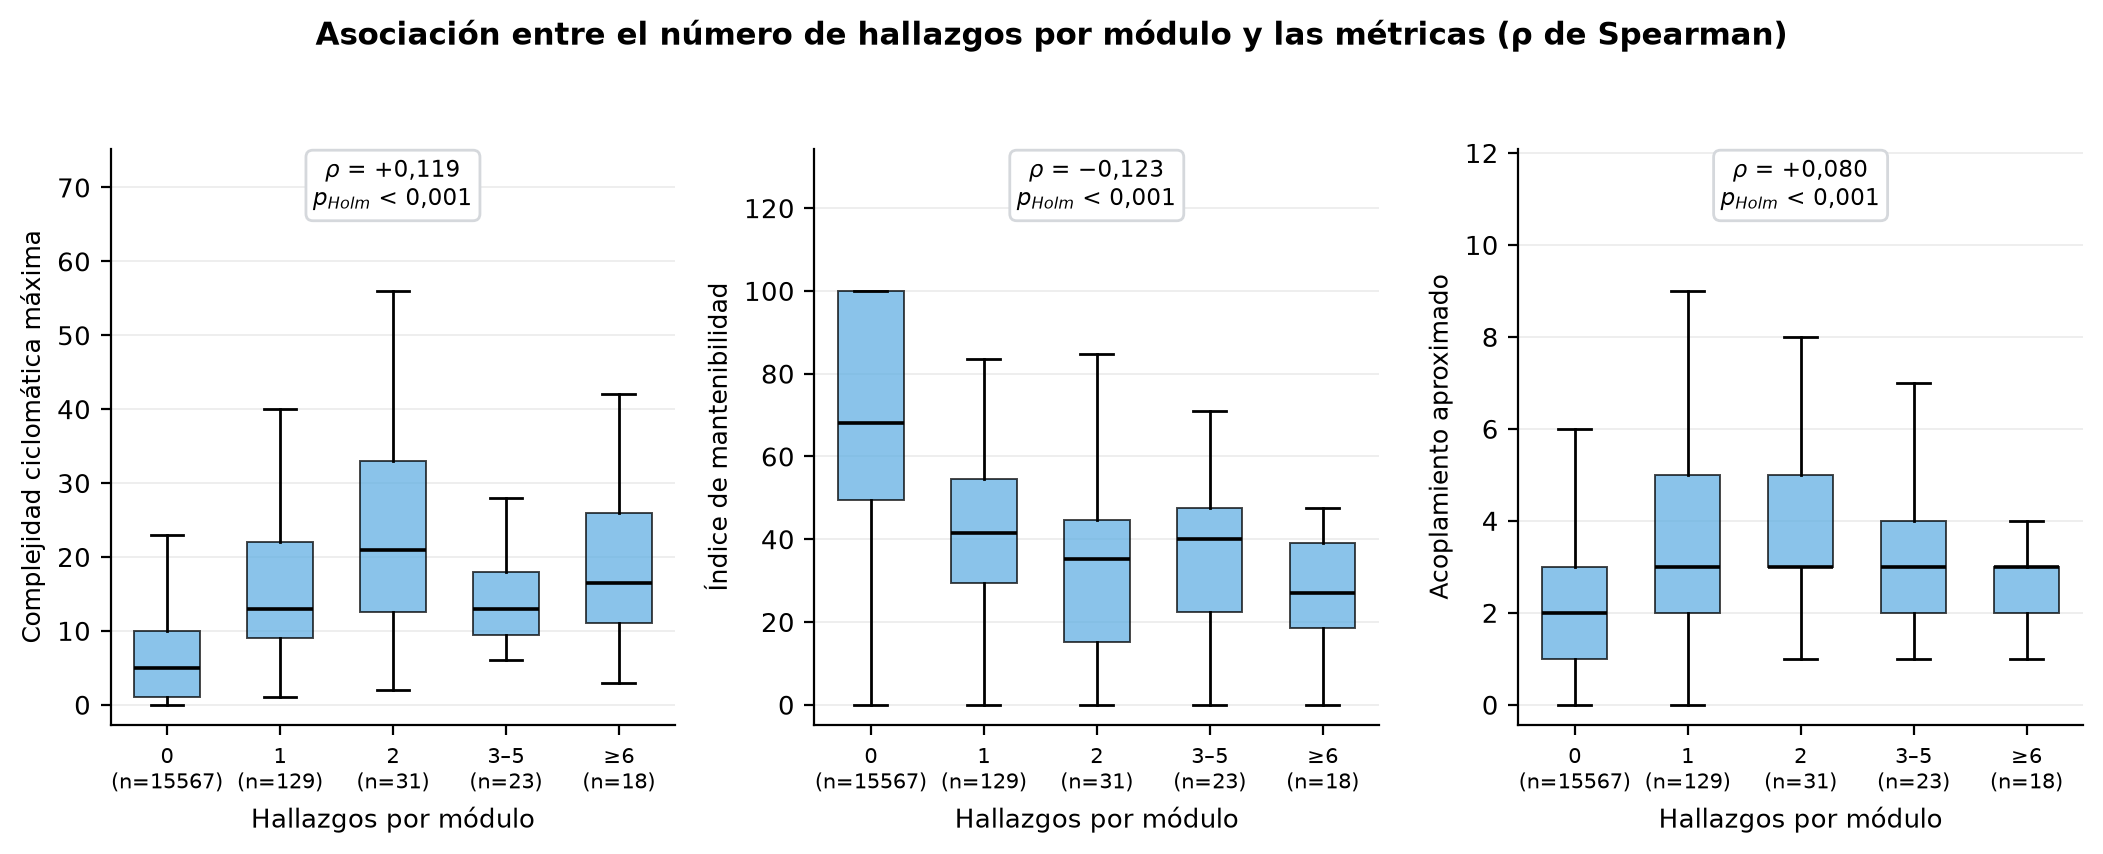
\includegraphics[width=0.95\textwidth]{figuras/fig06_correlacion_spearman.png}
\caption{Distribución de las métricas según el número de hallazgos por módulo. Los tamaños de grupo se indican en el eje horizontal; $\rho$ corresponde al coeficiente de Spearman sobre la variable de conteo completa.}
\label{fig:correlacion}
\end{figure*}

La diferencia entre el tamaño de efecto del contraste de grupos y la correlación merece atención. El $\delta$ de Cliff compara dos grupos y es grande para \texttt{cc\_max} y \texttt{mi}, mientras que $\rho$ es débil porque la mayoría de los módulos se concentra en cero y la variable de conteo tiene poca variación efectiva. Ambos resultados son compatibles: existe una separación entre \emph{tener} y \emph{no tener} antipatrones, pero el número de hallazgos por módulo no predice con precisión la magnitud de las métricas.

\subsection{Análisis por terciles de tamaño}

La Tabla~\ref{tab:terciles} y la Figura~\ref{fig:terciles} presentan el análisis exploratorio por terciles de \texttt{sloc}. El tercil inferior (hasta 43 líneas) contiene un solo módulo con antipatrón frente a 5313 sin antipatrón; por ello, sus valores se reportan pero no se interpretan inferencialmente y se marcan como \emph{n insuficiente}. El tercil medio (43--164 líneas) contiene 40 módulos con antipatrón y 5175 sin antipatrón; las tres métricas muestran diferencias significativas, con efecto mediano en \texttt{cc\_max} ($\delta=+0{,}391$) y efectos pequeños en \texttt{mi} ($\delta=-0{,}276$) y \texttt{cbo\_mod} ($\delta=+0{,}230$). El tercil superior (más de 164 líneas) contiene 160 módulos con antipatrón y 5079 sin antipatrón; \texttt{cc\_max} y \texttt{mi} mantienen efectos pequeños ($\delta=+0{,}270$ y $\delta=-0{,}306$), mientras que \texttt{cbo\_mod} presenta una diferencia estadísticamente significativa pero de efecto despreciable ($\delta=+0{,}142$), con medianas iguales a 3 en ambos grupos.

\begin{table*}[t]
\centering
\scriptsize
\setlength{\tabcolsep}{3.5pt}
\caption{Análisis exploratorio por terciles de líneas de código (SLOC)}
\label{tab:terciles}
\begin{tabularx}{\textwidth}{@{}l l l r r r r l r l >{\raggedright\arraybackslash}X@{}}
\toprule
\textbf{Tercil} & \textbf{SLOC} & \textbf{Métrica} & \textbf{n con} & \textbf{n sin} & \textbf{Med.\ con} & \textbf{Med.\ sin} & \textbf{p} & \textbf{$\delta$} & \textbf{Magnitud} & \textbf{Estado} \\
\midrule
Inferior & $\leq 43$ & \texttt{cc\_max} & 1 & 5\,313 & 1,00 & 1,00 & --- & $+0{,}184$ & Pequeño & \textit{n insuficiente} \\
 &  & \texttt{mi} & 1 & 5\,313 & 83,47 & 100,00 & --- & $-0{,}686$ & Grande & \textit{n insuficiente} \\
 &  & \texttt{cbo\_mod} & 1 & 5\,313 & 1,00 & 1,00 & --- & $+0{,}016$ & Despreciable & \textit{n insuficiente} \\
\midrule
Medio & 43--164 & \texttt{cc\_max} & 40 & 5\,175 & 8,50 & 5,00 & $1{,}87 \times 10^{-5}$ & $+0{,}391$ & Mediano & Significativo \\
 &  & \texttt{mi} & 40 & 5\,175 & 62,18 & 68,12 & 0,00257 & $-0{,}276$ & Pequeño & Significativo \\
 &  & \texttt{cbo\_mod} & 40 & 5\,175 & 2,00 & 2,00 & 0,00967 & $+0{,}230$ & Pequeño & Significativo \\
\midrule
Superior & $>164$ & \texttt{cc\_max} & 160 & 5\,079 & 15,50 & 12,00 & $5{,}46 \times 10^{-9}$ & $+0{,}270$ & Pequeño & Significativo \\
 &  & \texttt{mi} & 160 & 5\,079 & 35,09 & 43,69 & $4{,}17 \times 10^{-11}$ & $-0{,}306$ & Pequeño & Significativo \\
 &  & \texttt{cbo\_mod} & 160 & 5\,079 & 3,00 & 3,00 & 0,00186 & $+0{,}142$ & Despreciable & Significativo \\
\bottomrule
\end{tabularx}
\end{table*}

\begin{figure*}[t]
\centering
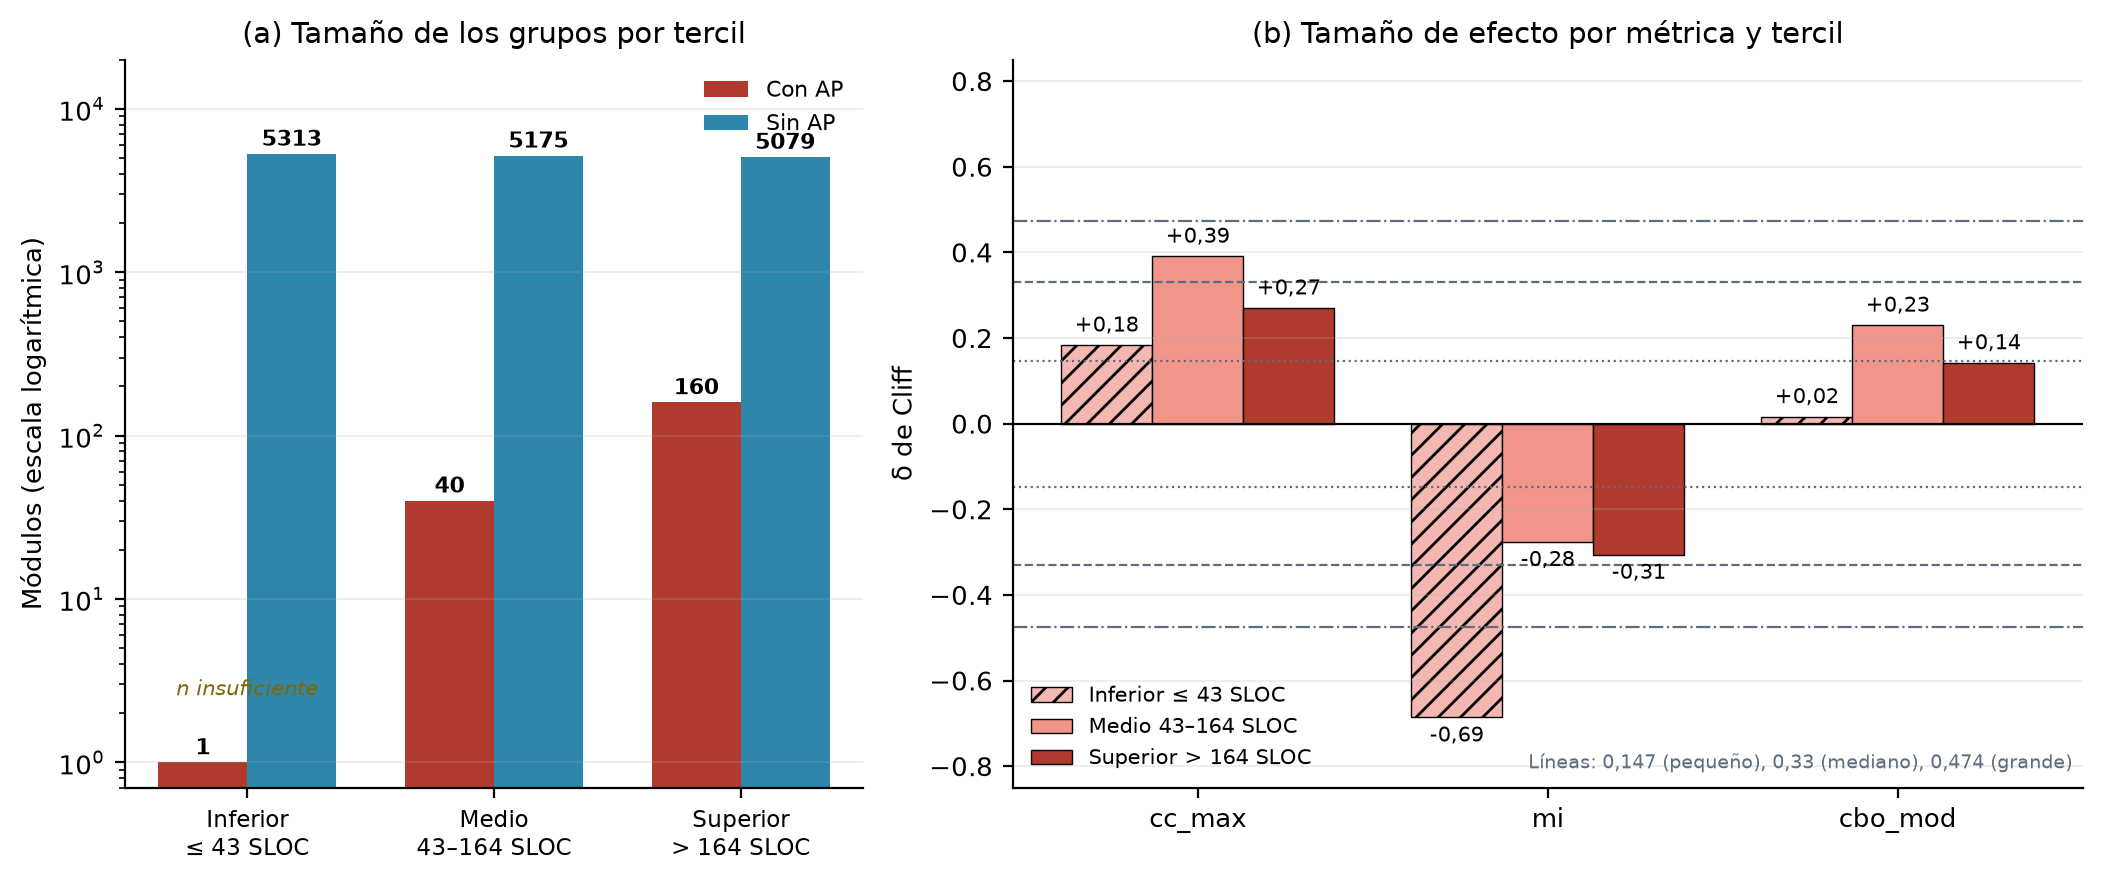
\includegraphics[width=0.92\textwidth]{figuras/fig07_terciles_sloc.png}
\caption{Análisis por terciles de líneas de código. (a) Tamaño de los grupos con y sin antipatrones en escala logarítmica. (b) Tamaño de efecto de Cliff por métrica y tercil; las barras rayadas corresponden al tercil inferior, con un solo módulo con antipatrón.}
\label{fig:terciles}
\end{figure*}

Estos resultados ofrecen evidencia parcial de que la asociación no se explica exclusivamente por el tamaño del código: dentro del tercil medio y del superior, las diferencias persisten en la dirección esperada para \texttt{cc\_max} y \texttt{mi}. Sin embargo, no la controlan por completo. El tercil superior sigue conteniendo módulos más grandes que el medio, y la estratificación por una sola variable no elimina la confusión residual por otras características del repositorio o del diseño. Además, los nueve contrastes por tercil son exploratorios y no fueron corregidos por multiplicidad; el valor $p=0{,}00186$ de \texttt{cbo\_mod} en el tercil superior debe leerse con cautela, sobre todo porque su tamaño de efecto es despreciable.

\subsection{Sensibilidad por repositorio}

La Tabla~\ref{tab:sensibilidad} presenta la comparación agregada de medianas por repositorio. Los 21 repositorios con hallazgos se comparan con los 2 repositorios sin hallazgos, un tamaño de grupo muy inferior al mínimo de cinco que el protocolo exige. Por esa razón, los tres contrastes se marcan como \emph{n insuficiente} y no se reportan valores $p$. Las diferencias descriptivas son mixtas: \texttt{cc\_max} es mayor en los repositorios con antipatrones (mediana 5 frente a 3,25; $\delta=+0{,}548$), lo que coincide con la dirección esperada; \texttt{mi} es ligeramente mayor en los repositorios con antipatrones (64,39 frente a 62,02; $\delta=+0{,}095$), en contra de lo esperado; y \texttt{cbo\_mod} es menor en los repositorios con antipatrones (2 frente a 2,25; $\delta=-0{,}452$), también en contra de lo esperado.

\begin{table*}[t]
\centering
\footnotesize
\setlength{\tabcolsep}{4pt}
\caption{Análisis de sensibilidad agregado por repositorio (medianas por repositorio)}
\label{tab:sensibilidad}
\begin{tabularx}{\textwidth}{@{}l r r r r r >{\raggedright\arraybackslash}X c l@{}}
\toprule
\textbf{Métrica} & \textbf{n con} & \textbf{n sin} & \textbf{Med.\ con} & \textbf{Med.\ sin} & \textbf{$\delta$} & \textbf{Dirección esperada} & \textbf{¿Coincide?} & \textbf{Estado} \\
\midrule
\texttt{cc\_max} & 21 & 2 & 5,00 & 3,25 & $+0{,}548$ & Mayor en con AP & Sí & \textit{n insuficiente} \\
\texttt{mi} & 21 & 2 & 64,39 & 62,02 & $+0{,}095$ & Menor en con AP & No & \textit{n insuficiente} \\
\texttt{cbo\_mod} & 21 & 2 & 2,00 & 2,25 & $-0{,}452$ & Mayor en con AP & No & \textit{n insuficiente} \\
\bottomrule
\end{tabularx}
\end{table*}

Este resultado no confirma ni refuta los hallazgos primarios. Lo que muestra es que la agregación por repositorio es demasiado frágil con dos observaciones en el grupo de comparación: un cambio en uno de esos dos repositorios puede invertir el signo. La sensibilidad por repositorio debe interpretarse como una advertencia sobre la dependencia de los resultados respecto de la composición de la muestra, no como una validación de robustez.

\subsection{Revisión asistida por inteligencia artificial}

La revisión de los 60 hallazgos muestreados produjo 21 propuestas de verdaderos positivos, 29 de falsos positivos y 10 casos indeterminados. La confianza declarada fue alta en 44 casos, media en 14 y baja en 2. La Tabla~\ref{tab:adjudicacion} desglosa estos valores por detector y la Figura~\ref{fig:adjudicacion} los ilustra. AP1 presenta 10 propuestas de verdaderos positivos, 6 de falsos positivos y 4 indeterminados; AP5 presenta 9, 7 y 4; AP3 presenta 1, 15 y 1; y AP4 presenta 1, 1 y 1. La lectura por detector debe hacerse con cautela porque el tamaño de la muestra es distinto en cada caso: AP3 y AP4 aportan todos sus hallazgos, mientras que AP1 y AP5 aportan veinte de sus respectivos totales.

Es fundamental no convertir estos valores en una tasa de precisión. El cociente 21/50 excluye arbitrariamente los 10 casos indeterminados y no cuenta con verificación humana independiente; además, la muestra está estratificada por detector y no es representativa de todos los hallazgos. Lo que puede afirmarse es que la revisión asistida por IA sugiere un riesgo considerable de falsos positivos, especialmente en AP3, donde 15 de 17 casos fueron propuestos como falsos positivos. Esta señal es coherente con la naturaleza heurística de las reglas y con la literatura sobre detección de olores, pero no constituye una medición de precisión.

\subsection{Síntesis de los resultados}

En conjunto, los resultados muestran cuatro patrones. Primero, los antipatrones implementados están presentes en la mayoría de los repositorios (21 de 23) y en una minoría de los módulos (201 de 15\,768). Segundo, la distribución está dominada por AP1 y AP5 y concentrada en dos repositorios. Tercero, los módulos con antipatrones presentan mayor complejidad, menor mantenibilidad y mayor acoplamiento aproximado, con tamaños de efecto grandes o medianos en el contraste de grupos y correlaciones débiles a nivel de conteo. Cuarto, el análisis por terciles sugiere que la asociación no se debe únicamente al tamaño del código, pero no la controla por completo, y la sensibilidad por repositorio es inconclusa. La revisión asistida por IA añade una advertencia sobre la posibilidad de falsos positivos que condiciona cualquier lectura de prevalencia.